
\chapter{Modelling of Multi-Rotor Aircraft}\label{chapter:Modelling}
\textit{In order to design a control system for an aircraft, a comprehensive mathematical model of the aircraft must first be defined. Within this chapter a complete state space representation is derived for a general multi-rotor vehicle. This model is then extended to a specific vehicle configuration - the hexacopter. This model is then simulated using Simulink in order to implement and test the control methods in the following chapter.}
\section{General Multi-Rotor Model}\label{section:MultiRotorModel}
The initial model will be derived for a general multi-rotor vehicle using Newton-Euler formalism. This is done by considering the torque around each of the three axes and the total force produced by the propellers as the inputs to the system. This model can then be extended to most standard multi-rotor configurations by considering how the propellers generate these forces and torques in the configuration being considered.


\subsection{Reference Frames}
We will consider a vehicle in three-dimensional space with six degrees of freedom (DoF)- three translational DoF (x, y and z), and three rotational DoF (roll $\phi$, pitch $\theta$ and yaw $\psi$). For the derivation of this model, it is necessary to consider two reference frames: the Earth-fixed frame and the body-fixed frame. The Earth-fixed local frame is that which has its origin at an arbitrary, stationary point on the Earth's surface, while the body-fixed frame originates at the vehicle's centre of mass and travels with the vehicle\cite{Nebylov2016}. The Earth-fixed frame will be considered an inertial frame for the purposes of this model. Note that in order to maintain right-hand orthogonality the inertial frame is traditionally defined with the positive x axis pointing North, the positive y axis pointing East and the positive z axis pointing down towards the Earth (known as North-East-Down (NED) co-ordinates). The NED reference frame is represented in \figref{fig:RefFrames} a) with axes ($x_{n}$, $y_{n}$, $z_{n}$). For the purposes of modelling an aerial vehicle it is more intuitive to have the z axis positive in the upward direction (corresponding to vehicle altitude).Therefore, a second inertial frame will be defined with axes ($x=x_{n}$, $y=y_{n}$, $z=-z_{n}$) as shown in \figref{fig:RefFrames} b). This reference frame will be referred to as the Earth frame and will be the main coordinate system used throughout this thesis. The body frame is defined with its origin at the vehicle's centre of mass with the z axis opposite to the direction of propeller thrust. The input torques ($\tau_{\phi}$, $\tau_{\theta}$, $\tau_{\psi}$) are defined around the axes of the body frame ($x_{b}$, $y_{b}$, $z_{b}$) as depicted in \figref{fig:RefFrames} c).\\


\begin{figure}[htb]
	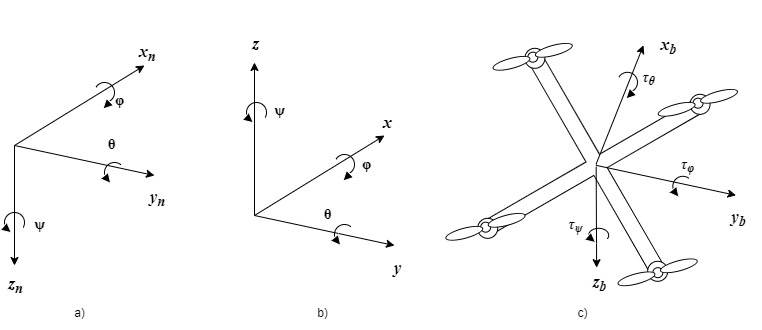
\includegraphics[width=\columnwidth]{RefFrames.jpg}%
	\caption{Reference frames and co-ordinate systems: a) NED Frame b) Earth Frame c) Body Frame}%
	\label{fig:RefFrames}%
\end{figure}

To transform linear quantities (displacement, velocity, acceleration) between the inertial NED coordinate system ($x_{n}, y_{n}, z_{n}$) and the body-fixed coordinate system ($x_{b}, y_{b}, z_{b}$) it is necessary to establish a rotation matrix ($C^{b}_{n}$) such that:
\[
\begin{bmatrix}
x_{b}\\ y_{b}\\ z_{b}
\end{bmatrix} = C^{b}_{n}\begin{bmatrix}
x_{n}\\ y_{n}\\ z_{n}
\end{bmatrix}
\]

To establish this matrix it is necessary to consider the rotation of the body-fixed frame around each of its axes\cite{Cook2013}. This is done by multiplying by three intermediate rotation matrices: $C^{b}_{n}(\phi)$, $C^{b}_{n}(\theta)$ and $C^{b}_{n}(\psi)$. Since matrix multiplication is not commutative, the order of these rotations is an important part of the model. The body frame is first rotated around the x axis (roll) by an angle $\phi$ to an intermediate reference frame: 
\[
\begin{bmatrix}
x_{b}\\ y_{b}\\ z_{b}
\end{bmatrix} = C^{b}_{n}(\phi)\begin{bmatrix}
x_{b_{1}}\\ y_{b_{1}}\\ z_{b_{1}}
\end{bmatrix}=
\begin{bmatrix}
1 & 0 & 0\\ 
0 & cos(\phi) & sin(\phi)\\ 
0 & -sin(\phi) & cos(\phi)
\end{bmatrix}
\begin{bmatrix}
x_{b_{1}}\\ y_{b_{1}}\\ z_{b_{1}}
\end{bmatrix}
\]
Rotating this set of coordinates around the y axis (pitch) will result in another intermediate reference frame:
\[
\begin{bmatrix}
x_{b_{1}}\\ y_{b_{1}}\\ z_{b_{1}}
\end{bmatrix} = C^{b}_{n}(\theta)\begin{bmatrix}
x_{b_{2}}\\ y_{b_{2}}\\ z_{b_{2}}
\end{bmatrix}=
\begin{bmatrix}
cos(\theta) & 0 & -sin(\theta)\\ 
0 & 1 & 0\\ 
sin(\theta) &  0 & cos(\theta)
\end{bmatrix}
\begin{bmatrix}
x_{b_{2}}\\ y_{b_{2}}\\ z_{b_{2}}
\end{bmatrix}
\]
Finally, this frame is rotated around the z axis (yaw):
\[
\begin{bmatrix}
x_{b_{2}}\\ y_{b_{2}}\\ z_{b_{2}}
\end{bmatrix} = C^{b}_{n}(\psi)\begin{bmatrix}
x_{n}\\ y_{n}\\ z_{n}\\
\end{bmatrix}=
\begin{bmatrix}
cos(\psi) & sin(\psi) & 0\\
-sin(\psi) & cos(\psi) & 0 \\ 
0 & 0 & 1\\ 
\end{bmatrix}
\begin{bmatrix}
x_{n}\\ y_{n}\\ z_{n}
\end{bmatrix}
\]
Therefore, via substitution, the multiplication of these three intermediate matrices gives the final rotation matrix- also commonly known as the Direction Cosine Matrix (DCM)\cite{Nebylov2016}:
\begin{align*}
C^{b}_{n} &= C^{b}_{n}(\phi)C^{b}_{n}(\theta)C^{b}_{n}(\psi)\\
&=\begin{bmatrix}
cos(\theta)cos(\psi) & cos(\theta)sin(\psi) & -sin(\theta)\\
sin(\phi)sin(\theta)cos(\psi)-cos(\phi)sin(\psi) & sin(\phi)sin(\theta)sin(\psi)+cos(\phi)cos(\psi) & sin(\phi)cos(\theta) \\ 
cos(\phi)sin(\theta)cos(\psi)+sin(\phi)sin(\psi) & cos(\phi)sin(\theta)sin(\psi)-sin(\phi)cos(\psi) & cos(\phi)cos(\theta)\\ 
\end{bmatrix}
\end{align*}


An important characteristic of this rotation matrix is its orthogonality, which implies its inverse is equal to its transpose i.e. $C^{n}_{b}=(C^{b}_{n})^{-1}= (C^{b}_{n})^{T}$.


\subsection{Model Dynamics}\label{section:ModelDynamics}
Standard configurations of multi-rotor vehicles consist of a number of propellers arranged symmetrically around the central body, all producing a force in the same direction. Therefore, regardless of the force produced by each individual propeller, the total thrust can only be produced in one direction which is aligned with the vehicle's vertical (z) axis. However, the differences in the forces produced by individual propellers will influence the rotational mechanics of the vehicle causing roll, pitch and yaw torques. 

This system is an under-actuated system, since there are six degrees of freedom (x, y, z, $\phi, \theta, \psi$) but only four effective inputs- the torque around each axis and the total thrust (\(\tau_{\phi},\tau_{\theta}, \tau_{\psi}, F_{T}\)). This means that it is not possible to directly affect two of the degrees of freedom. For example, assuming the body frame is initially aligned with the Earth frame, the two horizontal translational motions (x and y) can not be directly affected, as the thrust vector is aligned with the z axis. In order to cause translational motion in the x direction it is first necessary to change the pitch angle ($\theta$), which causes the thrust vector to have an x component. Likewise, to move in the y direction the roll angle ($\phi$) must first change. A mathematical model describing the motion of a multi-rotor vehicle will be derived in this section.\\

To obtain the rates of change of the Euler angles ($\dot{\phi}$, $\dot{\theta}$, $\dot{\psi}$) from the angular velocities around the body-fixed axes (p, q, r), it is necessary to use the intermediate rotation matrices \cite{Nelson1997}.


\begin{align*}
\begin{bmatrix}
p\\q\\r
\end{bmatrix}
&= C^{b}_{n}(\phi)C^{b}_{n}(\theta)
\begin{bmatrix}
0\\0\\\dot{\psi}
\end{bmatrix}
+C^{b}_{n}(\phi)
\begin{bmatrix}
0\\\dot{\theta}\\0
\end{bmatrix}
+
\begin{bmatrix}
\dot{\phi}\\0\\0
\end{bmatrix}\\
&=
\begin{bmatrix}
1 & 0 & -sin(\theta)\\
0 & cos(\phi) & sin(\phi)cos(\theta)\\
0 & -sin(\phi) & cos(\phi)cos(\theta)
\end{bmatrix}
\begin{bmatrix}
\dot{\phi}\\ \dot{\theta} \\ \dot{\psi}
\end{bmatrix}\\
\end{align*}

Taking the inverse of this matrix gives a set of expression for the rates of change of the Euler angles. 
\begin{equation}\label{eqn:state1}
\begin{bmatrix}
\dot{\phi}\\ \dot{\theta} \\ \dot{\psi}
\end{bmatrix} 
=
\begin{bmatrix}
1 & sin(\phi)tan(\theta) & cos(\phi)tan(\theta)\\
0 & cos(\phi) & -sin(\phi)\\
0 & sin(\phi)sec(\theta) & cos(\phi)sec(\theta)
\end{bmatrix}
\begin{bmatrix}
p\\q\\r
\end{bmatrix} 
\end{equation}


Next, the Newton-Euler equations of motion will be explored with respect to the body-fixed frame linear velocities (u, v, w) and angular velocities (p, q, r).
\begin{equation}\label{eqn:NewtEul1}
F=m\left(
\begin{bmatrix}
\dot{u}\\\dot{v}\\\dot{w}
\end{bmatrix}
+
\begin{bmatrix}
p\\q\\r
\end{bmatrix}
\times
\begin{bmatrix}
u\\v\\w
\end{bmatrix}
\right)
\end{equation}



For now it will be assumed the only forces acting on the vehicle are the vehicle's weight (in the positive direction of the NED frame z axis) and the total thrust produced by the propellers (in the negative direction of the body-fixed z axis). Substituting these forces into Equation \eqref{eqn:NewtEul1} and rearranging gives:
\begin{equation}\label{eqn:state2}
\begin{bmatrix}
\dot{u}\\\dot{v}\\\dot{w}
\end{bmatrix}
= 
\begin{bmatrix}
rv-qw-gsin(\theta)\\
pw-ru+gsin(\phi)cos(\theta)\\
qu-pv+gcos(\phi)cos(\theta)-\frac{1}{m}F_{T}
\end{bmatrix}
\end{equation}

Next, the rotational motion is considered:
\[
\begin{bmatrix}
\tau_{\phi}\\\tau_{\theta}\\\tau_{\psi}
\end{bmatrix}
=I_{b}
\begin{bmatrix}
\dot{p}\\\dot{q}\\\dot{r}
\end{bmatrix}
+ \begin{bmatrix}
p\\q\\r
\end{bmatrix}
\times
I_{b}
\begin{bmatrix}
p\\q\\r
\end{bmatrix}
\]
Where $I_{b}$ represents the vehicle's moment of inertia matrix. Assuming that the vehicle is symmetric about its axes, $I_{b}$ will be a diagonal matrix:
\[I_{b}=
\begin{bmatrix}
I_{xx} & 0 & 0\\
0 & I_{yy} & 0\\
0 & 0 & I_{zz}
\end{bmatrix}
\]
Rearranging for the derivatives of the angular velocities gives:
\begin{equation}\label{eqn:state3}
\begin{bmatrix}
\dot{p}\\\dot{q}\\\dot{r}
\end{bmatrix}
=
\begin{bmatrix}
\frac{I_{yy}-I_{zz}}{I_{xx}}qr+\frac{1}{I_{xx}}\tau_{\phi}\\
\frac{I_{zz}-I_{xx}}{I_{yy}}pr+\frac{1}{I_{yy}}\tau_{\theta}\\
\frac{I_{xx}-I_{yy}}{I_{zz}}pq+\frac{1}{I_{zz}}\tau_{\psi}
\end{bmatrix}
\end{equation}



Finally, it will be necessary to obtain the position of the vehicle with respect to the Earth reference frame. Therefore, the derivatives of the NED frame $x_{n}$, $y_{n}$ and $z_{n}$ positions are obtained by multiplying the rotational matrix $C^{n}_{b}$ by the body-fixed frame linear velocities (u, v and w). This gives \eqref{eqn:NEDvel}, with c() and s() representing cos() and sin() respectively. 
\begin{equation}\label{eqn:NEDvel}
\begin{bmatrix}
\dot{x}_{n}\\\dot{y}_{n}\\\dot{z}_{n}
\end{bmatrix}
=
\begin{bmatrix}
c(\theta)c(\psi) & s(\phi)s(\theta)c(\psi)-c(\phi)s(\psi) & c(\phi)s(\theta)c(\psi)+s(\phi)s(\psi)\\
c(\theta)s(\psi) & s(\phi)s(\theta)s(\psi)+c(\phi)c(\psi) & c(\phi)s(\theta)s(\psi)-s(\phi)c(\psi)\\
-s(\theta) & s(\phi)c(\theta) & c(\phi)c(\theta)
\end{bmatrix}
\begin{bmatrix}
u\\v\\w
\end{bmatrix}
\end{equation}

These velocities can then be converted into the Earth frame with the z axis pointing up, as shown in \eqref{eqn:state4}.
\begin{small}
\begin{equation}\label{eqn:state4}
\begin{bmatrix}
\dot{x}\\\dot{y}\\\dot{z}
\end{bmatrix}
=
\begin{bmatrix}
\dot{x}_{n}\\\dot{y}_{n}\\-\dot{z}_{n}
\end{bmatrix}
=
\begin{bmatrix}
c(\theta)c(\psi) & s(\phi)s(\theta)c(\psi)-c(\phi)s(\psi) & c(\phi)s(\theta)c(\psi)+s(\phi)s(\psi)\\
c(\theta)s(\psi) & s(\phi)s(\theta)s(\psi)+c(\phi)c(\psi) & c(\phi)s(\theta)s(\psi)-s(\phi)c(\psi)\\
s(\theta) & -s(\phi)c(\theta) & -c(\phi)c(\theta)
\end{bmatrix}
\begin{bmatrix}
u\\v\\w
\end{bmatrix}
\end{equation}
\end{small}

\eqref{eqn:state1}, (\ref{eqn:state2}), (\ref{eqn:state3}) and (\ref{eqn:state4}) comprise a complete state space model describing a general multi-rotor vehicle with 12 states. This state space model will be used for simulation of the multi-rotor.

It is important to note that although this model does not make any approximations, it does not necessarily consider every force the vehicle may be subject to. For example, the effects of wind, air friction and gyroscopic effects have not been considered in this model for simplicity. Also the dynamics of the motors and propellers have not yet been considered, only the torques and total force produced have been chosen as inputs.

\FloatBarrier
\subsection{Additional Translational Motion Equations}\label{section:AddTransMotion}
Although the model defined in Section \ref{section:ModelDynamics} is a complete state space model for the system, the translational motion is able to be represented in another form which will be useful for controllers defined in the following chapter. 
The only forces acting on the vehicle in the Earth frame are gravity in the negative z direction and the total thrust in the direction of the body frame z axis. This is expressed in \eqref{eqn:additionalState1}
\begin{equation}\label{eqn:additionalState1}
\begin{split}
F&=
\begin{bmatrix}
0\\0\\-mg
\end{bmatrix}
+
\begin{bmatrix}
c(\theta)c(\psi) & s(\phi)s(\theta)c(\psi)-c(\phi)s(\psi) & c(\phi)s(\theta)c(\psi)+s(\phi)s(\psi)\\
c(\theta)s(\psi) & s(\phi)s(\theta)s(\psi)+c(\phi)c(\psi) & c(\phi)s(\theta)s(\psi)-s(\phi)c(\psi)\\
s(\theta) & -s(\phi)c(\theta) & -c(\phi)c(\theta)
\end{bmatrix}
\begin{bmatrix}
0\\0\\-F_{T}
\end{bmatrix}\\
&=
\begin{bmatrix}
(-c(\phi)s(\theta)c(\psi)-s(\phi)s(\psi))F_{T}\\
(-c(\phi)s(\theta)s(\psi)+s(\phi)c(\psi))F_{T}\\
c(\phi)c(\theta)F_{T}-mg
\end{bmatrix}
\end{split}
\end{equation}

Using Newton's second law of motion ($F=ma$) in the Earth frame gives the second order differential equations in \eqref{eqn:additionalState2}
\begin{equation}\label{eqn:additionalState2}.
\begin{bmatrix}
\ddot{x}\\\ddot{y}\\\ddot{z}
\end{bmatrix}
=
\begin{bmatrix}
(-c(\phi)s(\theta)c(\psi)-s(\phi)s(\psi))\frac{F_{T}}{m}\\
(-c(\phi)s(\theta)s(\psi)+s(\phi)c(\psi))\frac{F_{T}}{m}\\
c(\phi)c(\theta)\frac{F_{T}}{m}-g
\end{bmatrix}
\end{equation}

\section{Hexacopter Model}
In order to extend the general multi-rotor model to a hexacopter, the six propeller forces need to be converted to the general model's inputs: three torques (around each axis) and one force (describing the total thrust). To achieve this, the configuration of the hexacopter must be defined. \figref{fig:hex} shows the basic geometry of a hexacopter platform with \(P_{1}, P_{2},...,P_{6}\) representing the six propellers. 

\begin{figure}[htb]
\begin{center}
	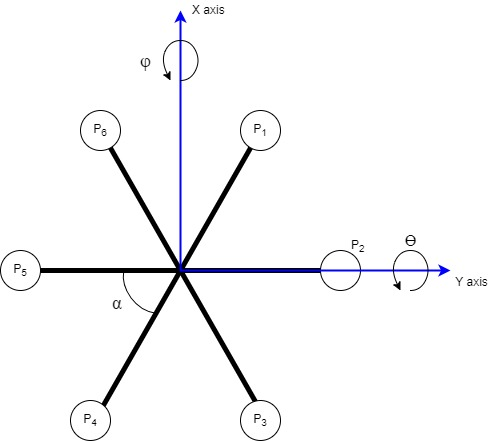
\includegraphics[width=90mm]{HexacopterConfig.jpg}%
	\end{center}
	\caption{Basic configuration of the hexacopter with labelled axes.}%
	\label{fig:hex}%
\end{figure}


Let \(F_{1}, F_{2},...,F_{6}\) denote the force produced by each of the propellers as numbered in \figref{fig:hex}. The torques around each axis are proportional to the distance of each propeller from the axis. Using the geometry of the hexacopter, the torques around each axis can be derived.
\begin{flushleft}
\[\tau_{\phi}=d[(F_{5}-F_{2})+\cos(\alpha)(F_{6}+F_{4}-F_{1}-F_{3})]\]\\
\[\tau_{\theta}=d\sin(\alpha)(F_{1}-F_{3}-F_{4}+F_{6})\]\\
\[\tau_{\psi}=K_{\psi}(F_{1}-F_{2}+F_{3}-F_{4}+F_{5}-F_{6})\]
\end{flushleft}
Where d represents the distance from each propeller to the hexacopter's centre of mass, \(\alpha\) represents the angle between each of the arms and K represents a constant arising from the reaction force on the propellers. In this case, the angles between each of the arms will be considered to be equal, therefore \(\alpha\) is 60\(^{\circ}\). It follows that \(\sin(\alpha)=\frac{\sqrt{3}}{2}\) and \(\cos(\alpha)=\frac{1}{2}\)\\

Next, it is necessary to express the torques in terms of the speed of the propellers. The force produced by the propellers is approximately proportional to the square of the speed of the propellers (\(\Omega_{i}^{2}\)). For now it is sufficient to relate the quantities with a constant (\(C_{T}\)) which is known to be related to the physical properties of the propeller and the medium in which it is rotating. These quantities are related by a different constant when considering the yaw torque (\(\tau_{\psi}\)) since this torque arises from reaction forces. The proportionality between the square of the propeller speeds and yaw torque will be represented by \(K_{\psi}\). The total thrust produced by the propellers (\(F_{T}\)) is simply the sum of the forces produced by each propeller. The relationship between the propeller speeds and input torques and force can thus be expressed in matrix form as in \eqref{eqn:propSpeeds1}.

\begin{equation}\label{eqn:propSpeeds1}
\begin{bmatrix}
\tau_{\phi}\\
\tau_{\theta}\\
\tau_{\psi}\\
F_{T}\\
\end{bmatrix}
=
\begin{bmatrix}
-\frac{C_{T}d}{2} & -C_{T}d & -\frac{C_{T}d}{2} & \frac{C_{T}d}{2} & C_{T}d & \frac{C_{T}d}{2}\\
    \frac{C_{T}d\sqrt{3}}{2} & 0 & -\frac{C_{T}d\sqrt{3}}{2} & -\frac{C_{T}d\sqrt{3}}{2} & 0 & \frac{C_{T}d\sqrt{3}}{2}\\
    K_{\psi} & -K_{\psi} & K_{\psi} & -K_{\psi} & K_{\psi} & -K_{\psi}\\
    C_{T} & C_{T} & C_{T} & C_{T} & C_{T} & C_{T}
\end{bmatrix}
\begin{bmatrix}
\Omega^{2}_{1}\\
\Omega^{2}_{2}\\
\Omega^{2}_{3}\\
\Omega^{2}_{4}\\
\Omega^{2}_{5}\\
\Omega^{2}_{6}\\
\end{bmatrix}
\end{equation}

It is also necessary to consider actuator saturation as part of this model. The motors which drive the propellers are limited in that they can only spin in a single direction and have a maximum speed output. That is, motor speeds $(\Omega_{1},\Omega_{2},\Omega_{3},\Omega_{4},\Omega_{5},\Omega_{6})$ are restricted such that:
\begin{equation}\label{eqn:saturation}
sat(\Omega_{i})=\begin{cases}
      \Omega_{max}, & \Omega_{i}>\Omega_{max}\\
      \Omega_{i}, & 0\leq\Omega_{i}\leq\Omega_{max}\\
      0, & \Omega_{i}<0
    \end{cases} 
\end{equation}
The block diagram of the final hexacopter model which combines \eqref{eqn:state1}, (\ref{eqn:state2}), (\ref{eqn:state3}), (\ref{eqn:state4}), (\ref{eqn:propSpeeds1}) and (\ref{eqn:saturation}) is shown in \figref{fig:FinalModel}.
\begin{figure}[htb]
\begin{center}
	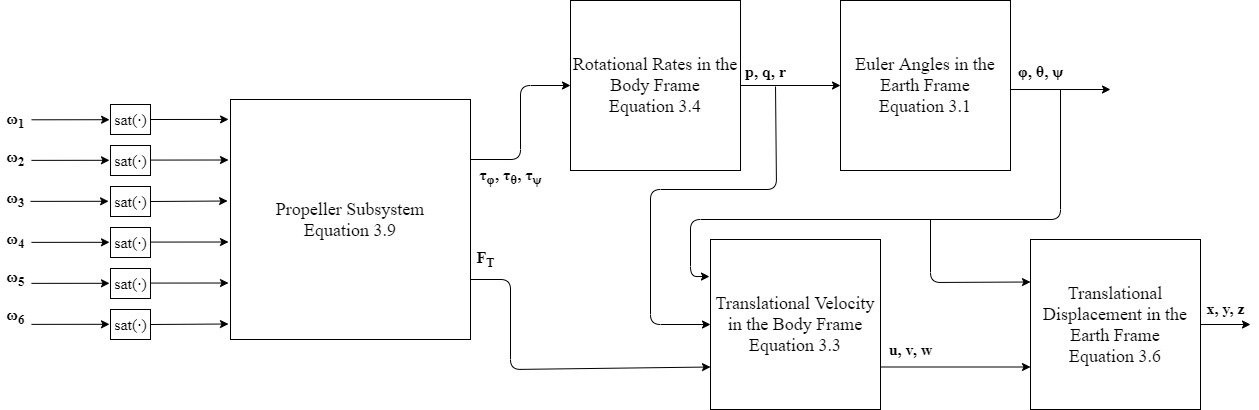
\includegraphics[width=\columnwidth]{ModelBlockDiagram.jpg}%
	\end{center}
	\caption{Hexacopter model block diagram.}%
	\label{fig:FinalModel}%
\end{figure}

 
\section{Simulation}
The model derived in the previous section is simulated using Simulink. The block diagrams created within Simulink are shown in Appendix \ref{section:Simu_Plant}.

The intent is to simulate the physical vehicle described in Section \ref{section:Hardware}. The vehicle's geometry and mass were measured, and are shown in \tabref{table:parameters} along with the other parameters used in the model. The maximum propeller speed was estimated based upon the voltage supplied by the battery and the manufacturer specifications. The propeller thrust coefficient was estimated, based upon the vehicles mass and the motors maximum speed. Since the vehicle is able to accelerate vertically, the thrust produced by the propellers must overcome the weight force, i.e. $C_{T}\Omega_{max}^{2}>mg$. Since more accurate methods were not readily available, a reasonable value of $C_{T}$ that satisfies this relationship was chosen. The yaw reaction torque coefficient was chosen to have the same order of magnitude as \cite{Bouabdallah2006} and \cite{Tayebi2004}. The moments of inertia around each axis are those measured for a similarly sized hexacopter using a pendulum by Capello et al. \cite{Capello2015}. These parameters do not exactly characterise the physical platform that is to be used, however the problem of parameter uncertainty is addressed in Section \ref{section:IntBack}.

\begin{table}[htb]\label{table:parameters}
\begin{center}
\begin{tabular}{||c|c|c|c||} 
 \hline
 Model Parameter & Symbol & Value & Units \\ [0.5ex] 
 \hline\hline
 Acceleration due to gravity & g & 9.81 & m s\textsuperscript{-2} \\ 
 \hline
 Vehicle mass & m & 1.404 & kg  \\
 \hline
 Moment of inertia (x) & I\textsubscript{xx} & 0.0286 & kg m\textsuperscript{2}\\
\hline
Moment of inertia (y) & I\textsubscript{yy} & 0.0254 & kg m\textsuperscript{2}\\
\hline
Moment of inertia (z) & I\textsubscript{zz} & 0.0418  & kg m\textsuperscript{2}\\
 \hline
 Angle between rotor arms & $\alpha$ & 60 & \textdegree\\
 \hline
 Maximum propeller speed & $\Omega_{max}$ & 252 & rev s\textsuperscript{-1}\\
 \hline
 Propeller thrust coefficient & $C_{T}$ & $4.5\times10^{-5}$ & N s\textsuperscript{2}\\
 \hline
 Yaw reaction torque coefficient & $K_{\phi}$ & $1.00\times10^{-7}$& N m s\textsuperscript{2}\\
\hline
 Distance from centre of gravity to propeller & d& 0.217 & m \\ [1ex] 
 \hline
\end{tabular}
\caption{Model simulation parameters}
\end{center}
\end{table}
 






\FloatBarrier
\section{Chapter Summary}
Within this chapter a complete state space representation has been derived to describe the dynamics of a general multi-rotor vehicle. This model has then been extended to a specific six rotor vehicle configuration. The simulation of the established model has been developed using Simulink. This simulated model will enable verification and testing of the control systems which are developed in the following chapter.
\clearpage


